\documentclass{beamer}
\usetheme{Madrid}

\usepackage{amsmath, amssymb, amsthm}
\usepackage{graphicx}
\usepackage{listings}
\usepackage{gensymb}
\usepackage[utf8]{inputenc}
\usepackage{hyperref}
\usepackage{gvv}

\begin{document}

\title{GATE-2022}
\author{EE23BTECH11016 - Aditi Dure$^{*}$}
\date{}
\frame{\titlepage}

\begin{frame}
\frametitle{Question}
%content
The block diagram of a two-tap high-pass FIR filter is shown below. The filter transfer function is given by $H(z) = \frac{Y(z)}{X(z)}$.\\
If the ratio of maximum to minimum value of $H(z)$ is 2 and $\abs{H(z)}_{max} = 1$, the coefficients $\beta_0$ and $\beta_1$ are \underline{\hspace{3cm}} and \underline{\hspace{3cm}}, respectively. 

\end{frame}

\begin{frame}
\frametitle{Block Diagram Given in Question}
%content
\begin{figure}[H]
    \centering
    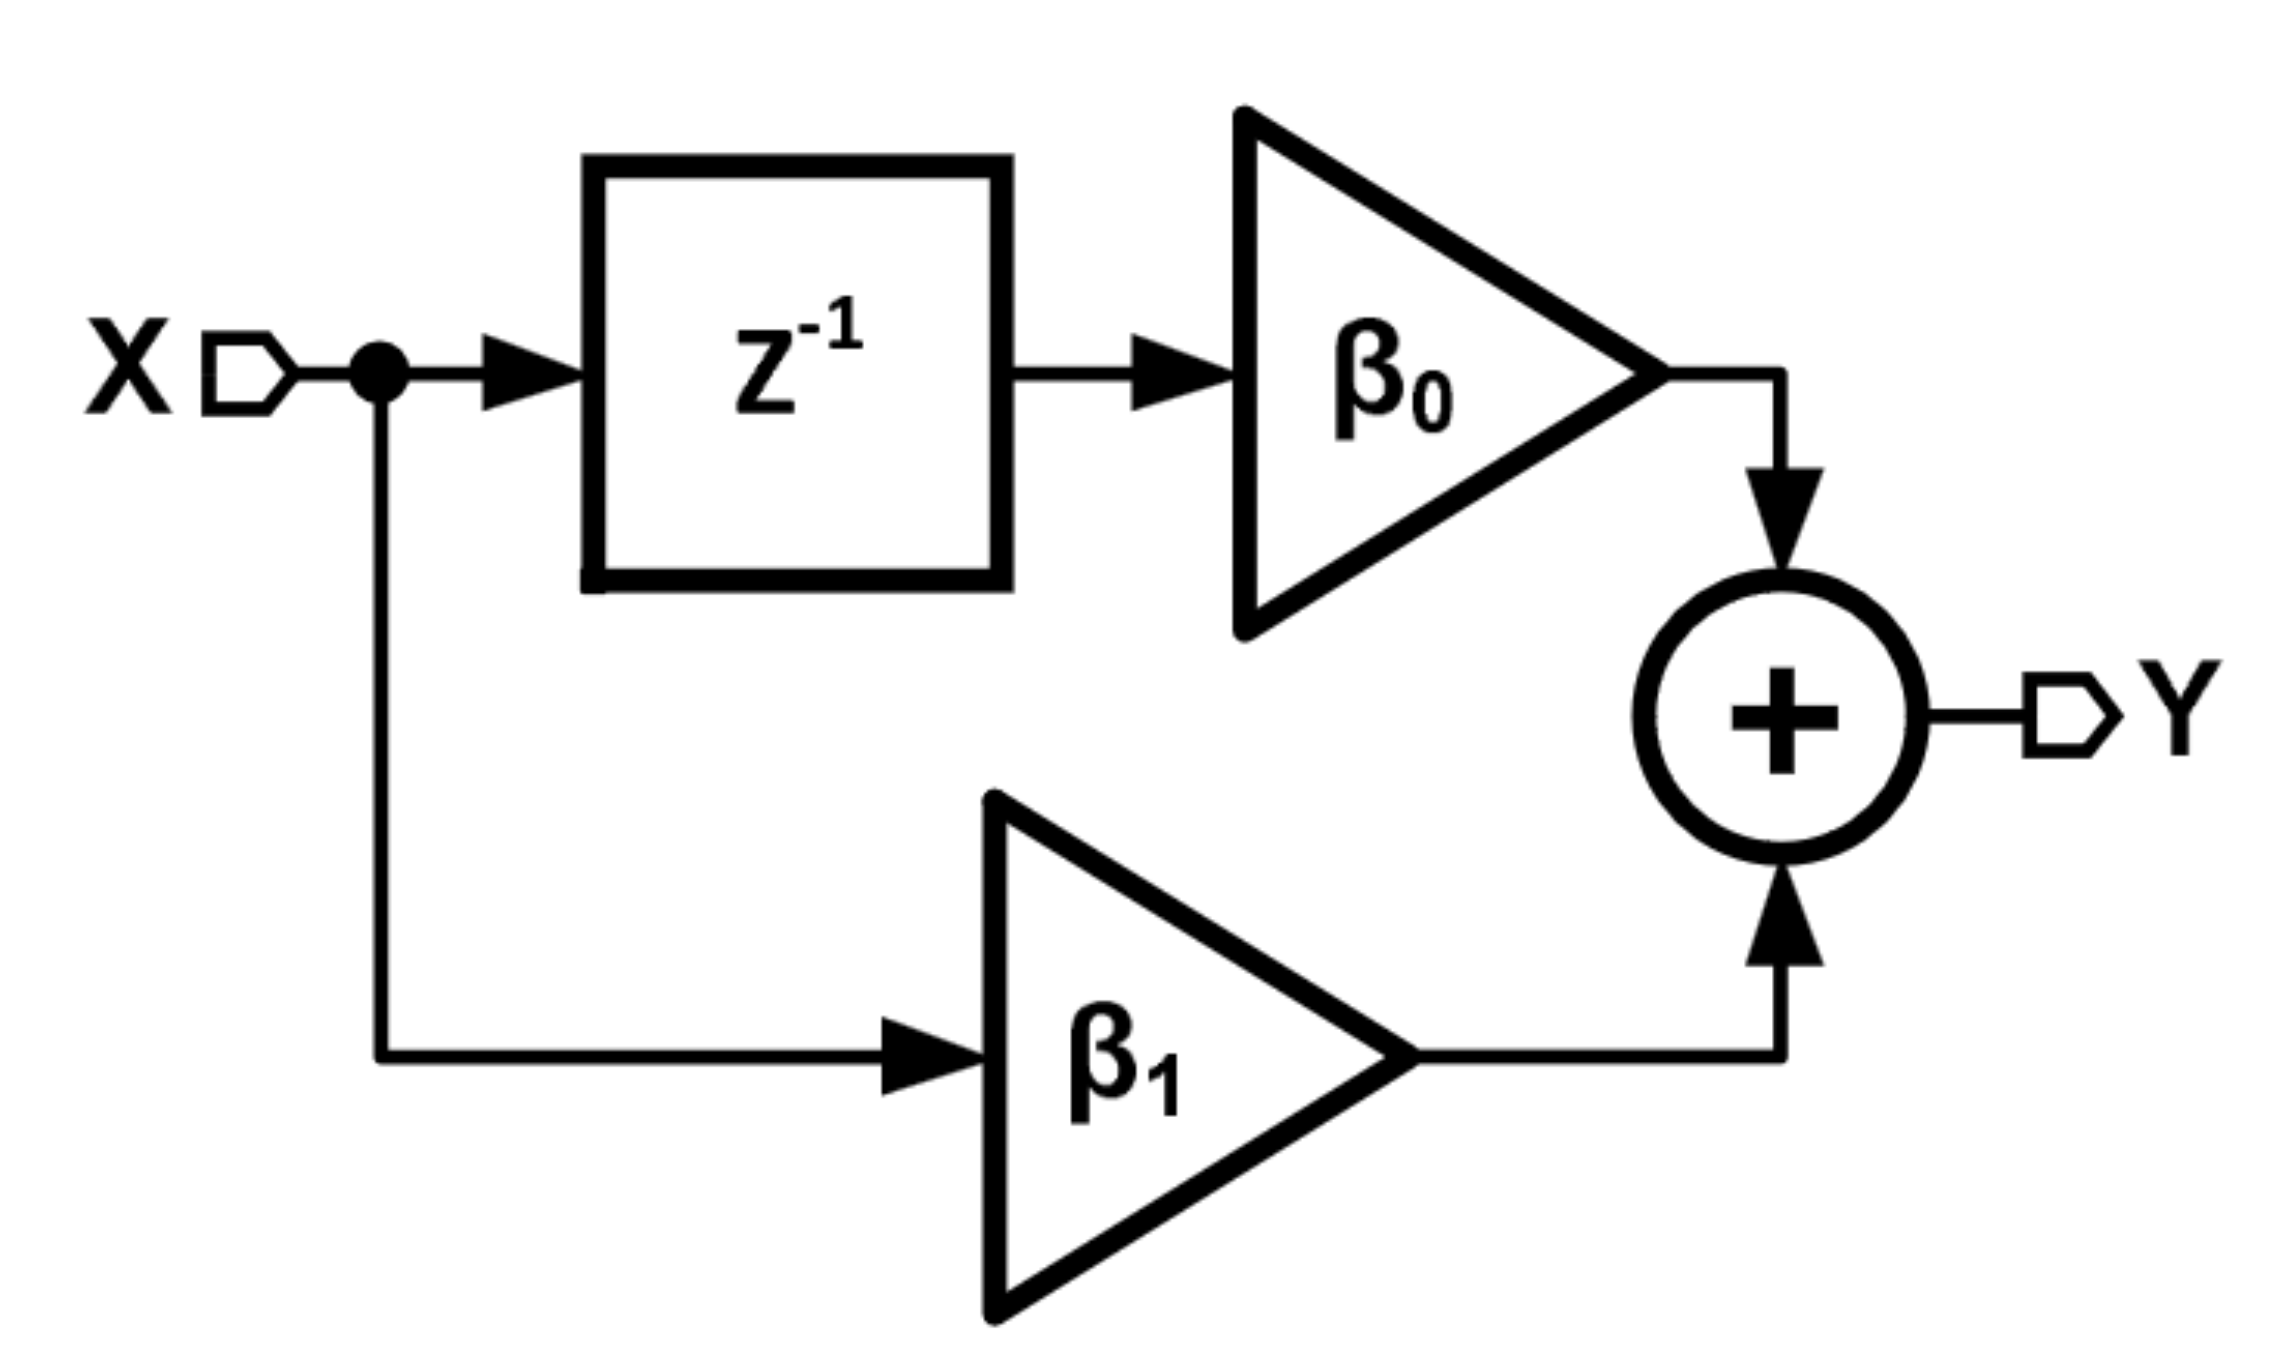
\includegraphics[width=0.5\linewidth]{figs/qfig.png} 
    \caption{Block diagram}
    \label{fig:GATE22BM39.1}
\end{figure}
\end{frame}

\begin{frame}
\frametitle{Options}
%content
\begin{enumerate}
\item 0.75, -0.25
\item 0.67, 0.33
\item 0.60, -0.40
\item -0.64, 0.36
\end{enumerate}
\hfill{GATE BM 2022}
\end{frame}

\begin{frame}
\frametitle{Results and Proofs}
%content
\underline{Time Shift Property:}
\begin{align}
x(n) &\overset{\mathcal{Z}}{\longleftrightarrow} X(z) \\
x(n-n_0) &\overset{\mathcal{Z}}{\longleftrightarrow} z^{-n_0}X(z) 
\end{align}
\end{frame}

\begin{frame}
\frametitle{Proof}
%content
Let
\begin{align}
y(n) &= x(n-n_0) \label{eq:GATE22BM39.-1}
\end{align}
Taking z-transform
\begin{align}
\mathcal{Z}\brak{y(n)} &= \mathcal{Z}\brak{x(n-n_0)} \label{eq:GATE22BM39.-2}
\end{align}
\end{frame}

\begin{frame}
\frametitle{Proof -- Continued}
%content
Simplifying LHS
\begin{align}
Y(z) &= \sum_{n=-\infty}^{\infty} y(n)z^{-n} 
\end{align}
From \eqref{eq:GATE22BM39.-1}
\begin{align}
Y(z) &= \sum_{n=-\infty}^{\infty} x(n-n_0) z^{-n} \label{eq:GATE22BM39.-3}
\end{align}
\end{frame}

\begin{frame}
\frametitle{Proof -- Continued}
%content
Let 
\begin{align}
n-n_0 = s  \implies
n = s+n_0 \label{eq:GATE22BM39.-4}
\end{align}
From \eqref{eq:GATE22BM39.-3} and \eqref{eq:GATE22BM39.-4}
\begin{align}
Y(z) &= \sum_{s=-\infty}^{\infty} x(s) z^{-(s+n_0)} \\
&= z^{-n_0}\sum_{s=-\infty}^{\infty} x(s) z^{-s} 
\end{align}
\end{frame}

\begin{frame}
\frametitle{Proof -- Continued}
%content
As variable in Z-transform is dummy, on replacing it, we get
\begin{align}
Y(z) &= z^{-n_0}\sum_{n=-\infty}^{\infty} x(n) z^{-n} \\
&= z^{-n_0}X(z) \label{eq:GATE22BM39.-5}
\end{align}
From \eqref{eq:GATE22BM39.-2} and \eqref{eq:GATE22BM39.-5}
\begin{align}
\mathcal{Z}\brak{x(n-n_0)} &= z^{-n_0}X(z)
\end{align}
\begin{center}
Hence Proved
\end{center} 
\end{frame}

\begin{frame}
\frametitle{Result}
%content
\begin{align}
z^{-n_0}X(z) &\overset{\mathcal{Z^{-}}}{\longleftrightarrow} x(n-n_0) \label{eq:GATE22BM39.-6}
\end{align}
\end{frame}



\begin{frame}
\frametitle{Conclusions}
%content
In \eqref{eq:GATE22BM39.-6}, put
\begin{align}
n_0 = 1, \quad x(n) = \delta(n) \nonumber 
\end{align}
Since
\begin{align}
1 \overset{\mathcal{Z^{-}}}{\longleftrightarrow} \delta(n) \nonumber
\end{align}
\begin{align}
z^{-1} &\overset{\mathcal{Z^{-}}}{\longleftrightarrow} \delta(n-1)
\end{align}
\end{frame}

\begin{frame}
\frametitle{Conclusions -- Continued}
%content
This is a unit delay in discrete time and represents unit amplitude sinosoidal signal.\\
So,
\begin{align}
z^{-1} &= e^{-jw} \\\implies
\abs{z^{-1}} &= 1 \label{eq:GATE22BM39.1}
\end{align}
\end{frame}


\begin{frame}
\frametitle{Solution -- Input Parameter Table}
%content
\begin{table}[h]
    \centering
        \begin{tabular}{|c|c|c|} 
      \hline
\textbf{Variable}& \textbf{Description}& \textbf{Value}\\\hline
	 $H(z)$ & Transfer Function & $\beta_0z^{-1} + \beta_1$ \\\hline
         $\abs{H(z)}_{max}$ & Maximum value of Transfer Function & 1 \\\hline  
         $\abs{H(z)}_{min}$ & Minimum value of Transfer Function & $\frac{1}{2}$\\\hline
    \end{tabular}

    \caption{input parameters}
    \label{tab:GATE22BM39.1}
\end{table}
\end{frame}


\begin{frame}
\frametitle{Solution -- Continued}
%content
Since $H(z)$ is complex, on using Triangle Inequality, we get
\begin{align}
\abs{x + y} \leq \abs{x} + \abs{y} 
\end{align}
And its corollary
\begin{align}
\abs{\abs{x}-\abs{y}} \leq \abs{x + y}
\end{align}
where x and y are complex numbers.
\end{frame}

\begin{frame}
\frametitle{Solution  -- Continued}
%content
\begin{align}
\abs{\abs{z^{-1}\beta_0}-\abs{\beta_1}} \leq \abs{z^{-1}\beta_0 + \beta_1} \leq \abs{z^{-1}\beta_0} + \abs{\beta_1} 
\end{align}
From \tabref{tab:GATE22BM39.1}
\begin{align}
\abs{\abs{z^{-1}\beta_0}-\abs{\beta_1}} \leq \abs{H(z)} \leq \abs{z^{-1}\beta_0} + \abs{\beta_1}
\end{align}
From \eqref{eq:GATE22BM39.1} 
\begin{align}
\abs{\abs{\beta_0}-\abs{\beta_1}} \leq \abs{H(z)} \leq \abs{\beta_0} + \abs{\beta_1} 
\end{align}
\end{frame}

\begin{frame}
\frametitle{Solution -- Continued}
%content
So, we can conclude that
\begin{align}
\abs{H(z)}_{max} &= \abs{\beta_0} + \abs{\beta_1} 
\end{align}
Now from \tabref{tab:GATE22BM39.1}
\begin{align}
1 &= \abs{\beta_0} + \abs{\beta_1} \label {eq:GATE22BM39.2}
\end{align}
Similarly,
\begin{align}
\frac{1}{2} &= \abs{\abs{\beta_0}-\abs{\beta_1}} \label {eq:GATE22BM39.3}
\end{align}
\end{frame}

\begin{frame}
\frametitle{Solution -- Continued}
%content
On solving \eqref{eq:GATE22BM39.2} and \eqref{eq:GATE22BM39.3}, we get
\begin{align}
\abs{\beta_0} = 0.75, \abs{\beta_1} = 0.25 
\end{align}
\begin{center}
OR
\end{center}
\begin{align}
\abs{\beta_0} = 0.25, \abs{\beta_1} = 0.75 
\end{align}
Hence the correct answer is option (A) \\
\end{frame}
\end{document}
